\documentclass[10pt,a4paper]{article}
\usepackage[utf8]{inputenc}
\usepackage{amsmath}
\usepackage{amsfonts}
\usepackage{amssymb}
\usepackage{amsthm}
\usepackage{graphicx}
\usepackage{stmaryrd}
\usepackage{url}
\usepackage{hyperref}
\newtheorem{thm}{Theorem}[section]
\newtheorem{lem}[thm]{Lemma}
\theoremstyle{plain}
\newtheorem{mydef}[thm]{Definition}
\theoremstyle{definition}
\newtheorem{myex}[thm]{Example}
\usepackage[english]{babel}
\author{Examples}

\begin{document}





\begin{figure}[h] \label{Laufband}
  \caption{In this example we have a robot moving on an infinite, discrete one-dimensional grid. Two players can control the robot, Player 0 and Player 1. The goal of Player 0 is to let the robot stay in the safe zone, the goal of Player 1 is to move the robot out of it. Both player take turns moving the robot, moving it at most one field in one direction.
.}
  \centering
    {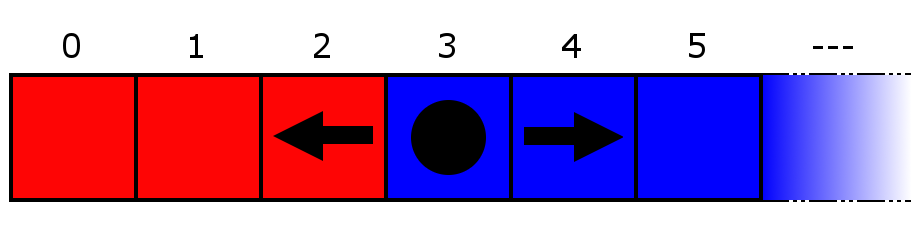
\includegraphics[width=8.0cm]{laufband.png}} 

\end{figure}


\begin{figure}[h]\label{Wassertank}
  \caption{Here we have a water tank and two players. This example works similiar to figure above, but this time the safe zone is limited by two sides since a water tank has only a finite capacity and we don't want the tank to run out of water.
}
  \centering
    {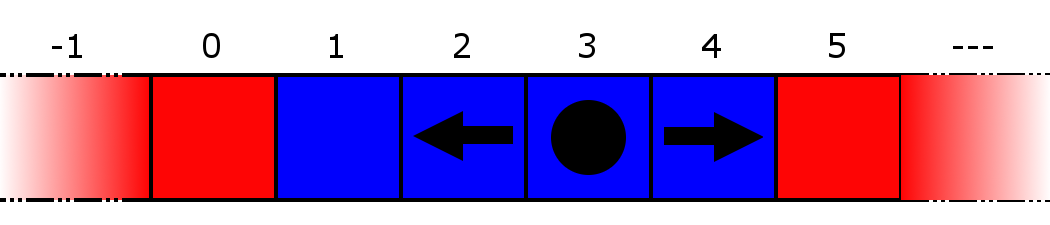
\includegraphics[width=8.0cm]{wasser_tank.png}} 
\end{figure}

\begin{figure}
  \caption{Consider a robot on an infinite two-dimensional grid with two players playing against each other. Both player can move the robot in an arbitrary direction by at most one field. Player 0 tries to keep the robot in a safe square, while Player 1 tries to move the robot out of the square.
}
  \centering
    {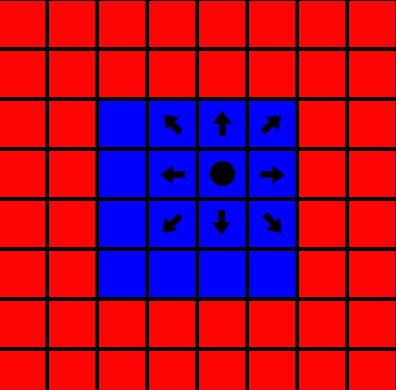
\includegraphics[width=8.0cm]{quadrat.png}} 
\end{figure}


\begin{figure}
  \caption{This example works like the water tank example, played with multiple tanks. Each player can control the tank in its turn and can decide to either fill the tank or empty the tank by one unit.}
  \centering
    {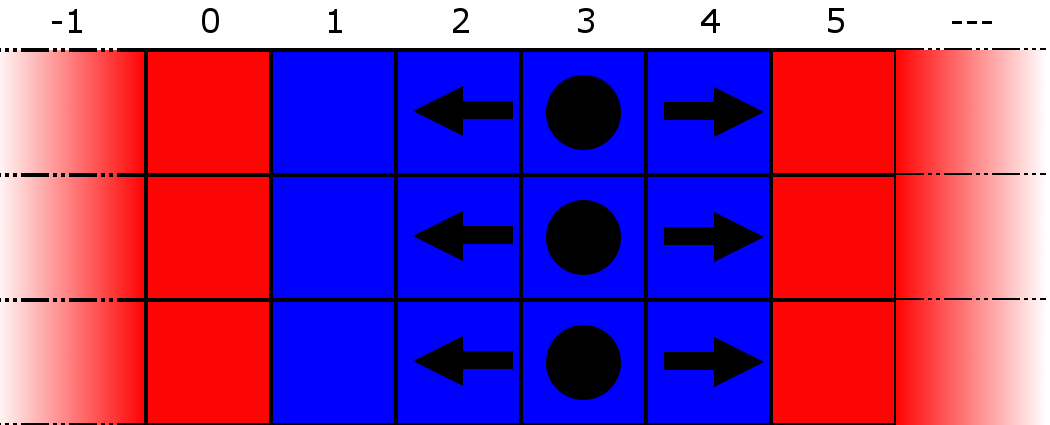
\includegraphics[width=8.0cm]{multi_wasser_tank.png}} 
\end{figure}






\begin{figure}
  \caption{In this example we have an infinite, discrete two-dimensional grid that is limited by two straight lines. Both player can move the robot in an arbitrary direction. Player 0 wins if the robot stays within the area limited by the straight lines. Player 1 wins if the robot moves out of it.}
  \centering
    {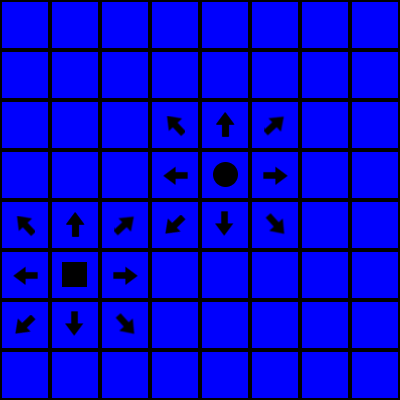
\includegraphics[width=8.0cm]{catch.png}} 
\end{figure}

\begin{figure}
  \caption{We have two robots moving in an infinite, discrete two-dimensional grid. Player 0's objective is to avoid being caught by Player 1.
}
  \centering
    {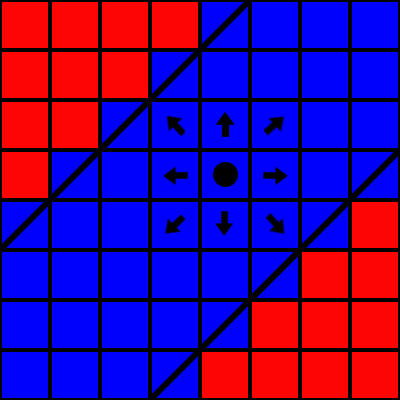
\includegraphics[width=8.0cm]{zwei_geraden.png}} 
\end{figure}

\end{document}